%!TEX root = Constructive Alignment for Introductory Programming.tex

\chapter{Introduction} % (fold)
\label{cha:introduction}

% Context, general problem, current solutions, why these solutions are still lacking, broadly what needs to be solved, my focus and research goal (something like that)

Programming is a critical skill in Computer Science and Software Engineering, as a consequence students in these fields are taught programming from the start of their degree programmes at many Universities. Although we have been teaching programming for a number of decades, learning programming remains challenging \cite{Jenkins:2002,Lister:2004,McCracken:2001,Ragonis:2007,Robins:2003,Rountree:2002,Renumol:2010,Wiedenbeck:2005}, with a general consensus that many students find programming hard. In fact, these challenges, and the current lack of success in this critical area, were recognied by \citet{McGettrick:2005} as one of their seven grand challenges in computing education. Despite persistent efforts over many years, we are still a long way from having specific guidance on how best to approach teaching introductory programming. Attempts in the field of computing education research have focused on curriculum, pedagogy, language choice, and tool support \cite{Pears:2007}. Further afield, advancements from general education literature provides additional advice on underlying theories and practices, including works on the scholarship of teaching and learning \cite{Boyer:1990}, approaches to teaching \cite{Martin:2000}, approaches to learning \cite{Marton:1976a,Trigwell:1999}, and analysis of the learner's experience \cite{Marton:1997}. 

% While seen as beneficial, these general education theories are seen as distant from the teaching of introductory programming, and there is a need for a greater inclusion of these topics in the computing education research discourse to help engage academics teaching \IP.

\rv{Approach towards teaching IP are diverse (TODO: provide some examples and cite). However, when considered in terms of students experience of learning to program\ldots} In their study of students' experiences learning to program, \citet{Bruce:2003} categorised the way students engage with learning to program into five categories range from approaches focusing on ``\emph{getting through the unit}'', to approaches aimed at discovering what it means to be a programmer. Each of these categories can be broadly classified as either a surface or deep approach to learning \cite{Marton:1976a,Ramsden:1992} to program. When engaging surface approaches, students attempt to address the outcomes with as little effort as possible. This leads to situations in which students are primarily motivated by fear of failing, and experience the learning as a struggle, with the topic appearing tedious, hard and boring. Adjectives that are often associated with learning to program. On the other hand, when engaging deep approaches to learning students seek meaning in what they do, and relate their learning to the bigger picture. To succeed at learning to program, students need to engage deep approaches to learning, as surface approaches alone are unlikely to be sufficient \cite{Bruce:2003}.

Biggs' model of \CA \cite{Biggs:1996c,Biggs:2007}, based upon constructive learning theory (constructivism) and aligned curriculum, aims to enhance student learning outcomes by focusing on \emph{what the student does}. \CA aims to encourage students to use \emph{deep}, rather than \emph{surface}, approaches to learning. Biggs' model is student focused, with clear and intentional alignment of assessment, teaching and learning activities, and unit objectives. The focus on the central role of the learner in building meaning is derived from constructivist learning theories \todo{cite}, whilst the alignment of assessment, teaching, and learning activities, has its foundation in instructional design literature \cite{Cohen:1987} \todo{cite more}.

As a form of outcomes based teaching and learning, \CA involves defining intended learning outcomes using verbs that indicate the required cognitive level students must engage. Assessment of student work is then carried out by evaluating the Structure of the Observed Learning Outcome (SOLO), using the SOLO Taxonomy developed by \citet{Biggs:1982}. \fref{constructive_alignment} illustrates the constructive alignment model presented by~\citet{Houghton:2004}, which consists of the following blocks:

\begin{itemize}
  \item \emph{Intended learning outcomes} clearly define required learning in terms of ``performances of understanding''.
  \item \emph{Performance objectives} emerge from the desired outcomes, and can be ranked to become the assessment criteria.
  \item \emph{Teaching and learning activities} are designed to place students in situations likely to elicit the required learning.
  \item Students provide \emph{evidence of their learning}, that is assessed against the criteria to determine grade outcomes.
\end{itemize}

\begin{figure}[htbp]
  \centering
  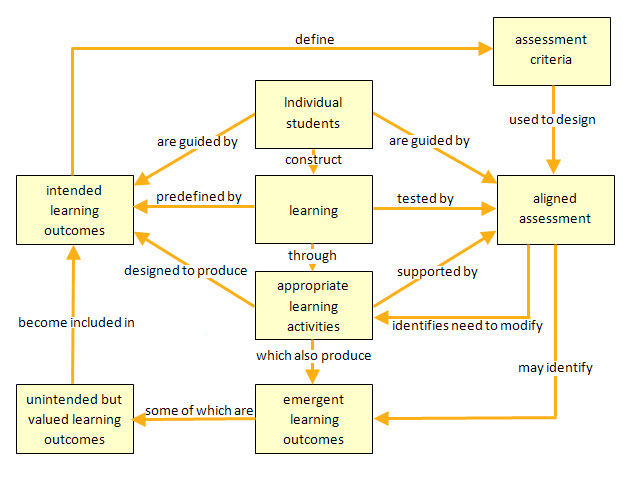
\includegraphics[width=\textwidth]{Houghton_constructive_alignment_1}
  \caption{Constructive alignment model presented by ~\citet{Houghton:2004}}
  \label{fig:constructive_alignment}
\end{figure}

While there is extensive literature on \CA in the general education literature, it has received little attention in computing eduction research related to teaching introductory programming. 

Given this contex, \todo{describe context}
Research that examines teaching environments is of great importance as it aids to build...


% - image on iterative nature of teaching

\section{Research Goals} % (fold)
\label{sec:research_goals}

This work will look to answer the following question. In what way can \emph{constructive alignment} be applied to the teaching of \emph{introductory programming} to stimulate \emph{deep approaches to learning}?

% To answer this question it is necessary to design and implement an introductory programming subject using the principles of constructive alignment. Designing such a subject requires the definition of intended learning outcomes, a statement of the assessment criteria, aligned teaching and learning activities, and a specific assessment approach. These activities require the following questions to be asked.

% \begin{enumerate}
%   \item What are appropriate intended learning outcomes?
%   \item Given the stated learning objectives, how can assessment criteria be structured to encourage students to use progressively deeper cognitive levels of activity in order to achieve higher grades? (memorise to reflect)
%   \item What teaching and learning activities help create an effective learning environment that encourages deep approaches to learning and a meaningful student experience?
%   \item How can criterion referenced assessment and holistic grading be used to assess student outcomes?
% \end{enumerate}

% To assess the effectiveness of the proposed teaching method the following questions will be addressed.

% \begin{enumerate}
%   \item Does this teaching method change the way students approach learning and/or their work in general?
%   \item What affect does this teaching method have on student engagement?
%   \item Are students able to effectively select material to demonstrate coverage of the intended learning outcomes?
%   \item To what depth does submitted work demonstrate the intended learning outcomes?
%   \item To what degree are students able to correctly assess their work against the subject's assessment criteria?
%   \item How well do students retain the knowledge and skills they develop in the subject?
% \end{enumerate}

% % Improve depth of learning.
% % 
% % Our method of teaching with constructive alignment: 
% % \begin{itemize}
% %   \item Determine learning objectives
% %   \item Create tiered assessment criterion that provide requirements for differing depths of understanding...
% %   \item Make students responsible for as much of their learning as possible. It is what they do that counts.
% %   \item Teach programming, not the language. Focus lectures on concepts and abstractions, provide just enough syntax to get the students started.
% %   \item Provide resources for students to learn the required syntax to map concepts to code (podcasts, text) to allow them to learn independently.
% %   \item Provide regular formative feedback on assessment work
% %   \item Have students prepare a portfolio of their work that demonstrates how they have addressed the assessment criteria
% % \end{itemize}
% % 
% % \bigskip
% % 
% % Guiding principles:
% % \begin{itemize}
% %   \item Truth. Remain true to the language and how it should be used. Avoid half truths as much as possible.
% %   \item Trust. Students are there to learn. They are capable and just need direction, encouragement, and feedback. Theory Y.
% %   \item Construct knowledge. Introduce the concepts needed to fully\footnote{Fully at this level of abstraction.} understand the programs they are writing. Avoid all forms of `magic'.
% %   % \item Students should use deep approaches to learning.
% %   % \item Programs are not sufficient to assess the depth of a students understanding.
% %   \item Maintain a good signal to noise ratio. Provide the essential material and have students explore the details themselves.
% %   \item Encourage deep exploration once concepts are grasped. For example, encourage students to look at how programming mechanisms work like how parameter passing works, how the stack grows, how a program's memory is organised.
% %   \item Flexible delivery with clear learning outcomes that allow students to customise the learning experience to their own needs and interests.
% %   \item Self efficacy allowing students to work toward a grade.
% % \end{itemize}
% % 
% % \clearpage

% % In what way can \emph{constructive alignment} be applied to the teaching of \emph{introductory programming} to stimulate \emph{deep learning}?

% % (Breadth vs depth)
% % 
% % What are the benefits of \emph{constructive alignment} for the teaching of \emph{introductory programming}?
% % 
% % What is the impact of \emph{constructive alignment} on overall computer science curriculum?
% % 
% % Does \emph{constructive alignment} encourage \emph{deep approaches to learning} in introductory programming subjects?




% % \begin{enumerate}
% %   \item How have other educational areas implemented constructive alignment?
% %   
% %   \item What are appropriate learning objectives for an introductory programming subject?
% %   \begin{itemize}
% %     \item What are the related programming concepts and abstractions?
% %     \item Are there established models of these concepts and abstractions?
% %     \item How do the concepts and abstractions map to different programming paradigms and languages?
% %     \item Which of these concepts and abstractions are appropriate for introductory programming subjects? What are the differences for subjects that use an `Objects First' approach versus an `Objects Later' approach? How do the two approaches compare on concept and abstraction coverage?
% %   \end{itemize}
% %   
% %   \item Given the selected learning objectives, how can assessment criteria be structured to encourage students to demonstrate use of progressively deeper cognitive levels in order to achieve higher grades? (memorise to reflect)
% %   \begin{itemize}
% %       \item What are the different cognitive levels of activities related to programming? (Is programming really `application' or just `expression'? e.g. getting it to work does even mean the student can explain why/how it works.) How do these relate to deep and surface approaches? How does this map to the SOLO taxonomy. (Is there work related to this?)
% %     % \item Can tiered assessment criteria be developed to map student outcomes to grade categories for use in criterion referenced assessment? How can these be formulated to encourage students to engage deeper learning approaches for higher grades?
% %     \item Are students aware of what is required to achieve different grades, and how does this change during the semester?
% %     \item What affect does the tiered assessment criteria and criterion referenced assessment have on student approaches to learning?
% %     \item Do students use criterion referenced assessment to customise the learning experience to their own requirements,  interests, and aspirations?
% %     \item Does this self directed learning and self efficacy help motivate students? Does this in turn lead to deeper approaches to learning and deeper learning outcomes?
% %     \item How do student aspirations change as the semester progresses? 
% %   \end{itemize}
% %   
% %   % \item What teaching and learning activities can help support the students to studying sound combination of theory and practice.
% %   % \item What benefits are there from providing flexible teaching and learning activities that align with the selected learning outcomes?
% %   % \item Given the selected learning outcomes, what are the benefits of providing flexible teaching and learning activities?
% %   % \item What teaching and learning activities that support and motivate
% %   % 
% %   % \item What teaching and learning activities help support student self-directed leaning of the conten
% %   % 
% %   % \item Can innovative teaching and learning activities encourage students to use deep approaches to learning?
% %   % 
% %   % \item Given the learning objective and assessment criteria, what teaching and learning activities are effective/ineffective?
% %   % 
% %   % \item What do students find useful about the teaching and learning activities used?
% %   
% %   % \item What teaching and learning activities can create an effective learning environment and a meaningful student experience?
% %   
% %   \item What teaching and learning activities help create an effective learning environment and meaningful student experience?
% %   \begin{enumerate}
% %     \item How can we make more effective use of lecture time? 
% %     \item Can we focus on programming concepts and abstractions at a higher level and use other means to cover details of language syntax?
% %     \item Can language syntax be covered sufficiently if the lecture focus shifts toward concepts?
% %     \item What effect does this have on student learning outcomes, sense of achievement, and learning approach?
% %     \item Are video podcasts an effective means of demonstrating programming abstractions and syntax?
% %     \item Does the focus on concepts help students learn a second programming language? How?
% %     \item How much overhead is there in switching between languages?
% %     \item Can you effectively teach programming using multiple languages in the one subject? What are the advantages and disadvantages of this?
% %     \item How does covering multiple languages impact on the student's learning experience?
% %     
% %     \item Will students use a focused episodic text? (??)
% %     % \item Motivation (Dan Pink, Motivation)
% %     \item Self determination (efficacy)
% %   \end{enumerate}
% %   
% %   % Holistic, 
% %   % Formative assessment during the semester
% %   
% %   \item How can criterion referenced assessment and holistic grading be used as assess student outcomes in introductory programming subjects?
% %   % \item Can portfolio assessment be used effectively for assessing student outcomes in introductory programming subjects?
% %   \begin{enumerate}
% %     \item What benefits are there from this approach to assessment and grading?
% %     \begin{itemize}
% %       \item Self efficacy?
% %       \item Deep learning outcomes?
% %     \end{itemize}
% %     \item What mechanisms can be introduced to limit plagiarism?
% %     \item Does the use of ungraded formative assessment during semester reduce plagiarism?
% %     \item Are students able to grasp the 
% %     \item What strategies work effectively for providing frequent formative feedback for large classes?
% %     \item What about the portfolio assessment approach encourages or discourages plagiarism? What mechanisms can be put in place to further discourage plagiarism?
% %     
% %     \item How are student portfolios affected by the statement of the assessment criteria?
% %     \item Does criterion referenced assessment alter the way students approach study in the subject?
% %     \item Does criterion referenced assessment alter the way students approach study in other subjects?
% %     \item Does their approach to portfolio assessment change in subsequent subjects that use the same approach? How? How do these changes (if there are any) relate to deep approaches to learning?
% %     \item Can portfolio assessment be scaled to larger class sizes?
% %   \end{enumerate}
% %   
% %   \item How do student approaches to learning change over time?
% %   \begin{enumerate}
% %     \item During the semester
% %     \item Over the year
% %     \item Across the course
% %     \item After uni
% %   \end{enumerate}
% %   
% %   \item What makes this an effective or ineffective method of teaching introductory programming?
% %   \item What effect does this teaching method have on student graduate attributes? (communication, problem solving, etc.)
% %   
% % \end{enumerate}
% % 
% % Objective:
% % \begin{enumerate}
% %   \item Model of programming concepts and abstractions, with multiple views for different language and paradigms.
% %   \item Guidelines on programming concepts applicable for introductory programming.
% %   \item Guidelines for building tiered assessment criteria.
% %   \item Guidelines, support for, benefits of constructive alignments etc.
% %   \item Behaviour tree for diagnostic view when students incorrectly self assess their grade - what was the cause. Student incorrectly self assessed -> over/under -> etc. Vs our expectations vs assessment criteria (grade)
% % \end{enumerate}

% section research_goals (end)


\section{Research Approach} % (fold)
\label{sec:research_approach}

% Research Questions and Method

% section research_approach (end)


\section{Key Findings} % (fold)
\label{sec:key_findings}

% Key Findings - page

% section key_findings (end)


\section{Thesis Structure} % (fold)
\label{sec:thesis_structure}

% Thesis Structure - para for each chapter

% section thesis_structure (end)


% chapter introduction (end)

